\documentclass[11pt,a4paper]{article}

\usepackage[margin=1in]{geometry}
\usepackage{titlesec}
\usepackage{enumitem}
\usepackage{hyperref}
\usepackage{parskip}
\usepackage{graphicx}
\usepackage{float}
\usepackage{booktabs}
\usepackage{amsmath}
\usepackage{amssymb}

\hypersetup{colorlinks=true, linkcolor=blue, urlcolor=blue}

\titleformat{\section}{\large\bfseries}{\thesection}{0.5em}{}
\titleformat{\subsection}{\normalsize\bfseries}{\thesubsection}{0.5em}{}
\setlist{leftmargin=1.4em, topsep=2pt, itemsep=2pt}

\title{\vspace{-1.5cm}\textbf{PKCERT AI \& Software Development Internship \\ Task 25: Sequence Modeling -- RNN/LSTM Fundamentals \& Text Classification}}
\author{Abdullah Amir}
\date{AI and Software Development \\ 10 August 2026}

\begin{document}

\maketitle
\vspace{-0.8cm}

Full code lives in \texttt{Day\_25.ipynb} and the standalone scripts it is built from.
\textbf{NumPy only} for every Part A/B derivation and the manual LSTM cell (no autograd
framework) -- \textbf{PyTorch 2.13.0 (CPU-only build)} used solely to verify the manual LSTM
cell against \texttt{nn.LSTMCell} and to train the Part C classifier, random seed
\textbf{42} fixed throughout. Every backward pass below is derived by hand and then verified
-- against numerical gradient checking or a known-correct PyTorch reference -- before being
trusted.

% ----------------------------------------------------------------
\section*{Part A: Sequence Data \& RNN Fundamentals}

\textbf{A1 -- sequential vs.\ i.i.d.\ tabular data.} A tabular dataset is modeled as i.i.d.:
the joint likelihood factorizes as $\prod_i P(x_i,y_i)$, so row order carries no information.
Sequential data (text, time series, audio) violates this on two counts: (1) order carries
information the model must use -- ``dog bites man'' vs.\ ``man bites dog'' -- and elements are
conditionally dependent, $P(x_t \mid x_{<t}) \neq P(x_t)$ in general; (2) sequences have
variable length, whereas tabular rows share a fixed feature dimensionality by construction.
\textbf{Feedforward networks are structurally unsuited}: an MLP $y=f(Wx+b)$ needs a
fixed-size input and has no mechanism to use position or history -- flattening to a fixed
length hard-codes a maximum length and gives each position an \emph{independent} weight set
(no parameter sharing across positions), while pooling discards order entirely. Neither lets
the network learn one position-independent update rule for combining new information with
history, which is exactly what an RNN provides via a shared recurrent weight matrix.

\textbf{A2 -- vanilla RNN recurrence, matrix form.} For input $x_t \in \mathbb{R}^d$, hidden
state $h_t \in \mathbb{R}^H$, output $y_t \in \mathbb{R}^C$:
$$h_t = \tanh(W_{xh} x_t + W_{hh} h_{t-1} + b_h), \qquad y_t = W_{hy} h_t + b_y$$
with $W_{xh}\in\mathbb{R}^{H\times d}$, $W_{hh}\in\mathbb{R}^{H\times H}$, $b_h\in\mathbb{R}^H$,
$W_{hy}\in\mathbb{R}^{C\times H}$, $b_y\in\mathbb{R}^C$ -- the \emph{same} five parameters
reused at every time step. Verified programmatically: a from-scratch NumPy
\texttt{VanillaRNNCell} run on a $(T{=}7, d{=}10)$ input produces hidden states of shape
$(7,16)$ and outputs of shape $(7,4)$ for $H{=}16, C{=}4$, matching this derivation exactly.

\textbf{A3/A4 -- BPTT and the Jacobian-product origin of vanishing/exploding gradients.}
Unrolling the recurrence across $t=1..T$ turns it into a $T$-layer graph sharing $W_{hh}$ at
every layer. For a loss $L$ depending on $h_T$, the gradient w.r.t.\ an earlier hidden state
$h_k$ is a \emph{product} of $(T-k)$ Jacobians:
$$\frac{\partial L}{\partial h_k} = \frac{\partial L}{\partial h_T} \prod_{t=k+1}^{T} \mathrm{diag}(1-h_t^2)\,W_{hh}$$
If the largest singular value of $\mathrm{diag}(1-h_t^2)W_{hh}$ is consistently $<1$, this
product shrinks \emph{geometrically} in $(T-k)$ -- vanishing gradients; if consistently $>1$,
it grows geometrically -- exploding gradients. The gradient w.r.t.\ the shared weight itself
sums this effect over every time step it was used:
$\;dL/dW_{hh} = \sum_{t=1}^{T} (dL/dh_t)(h_{t-1})^\top$, where each $dL/dh_t$ already contains
a Jacobian product back to every earlier $h_k$. \textbf{Long-range dependencies are hard}
because the terms in this sum from small $t$ (early steps) are exactly the ones multiplied by
the longest, most attenuated Jacobian products -- the gradient signal that would teach
$W_{hh}$ to exploit an early-input/final-loss dependency is systematically the smallest term
in the sum.

\begin{figure}[H]
    \centering
    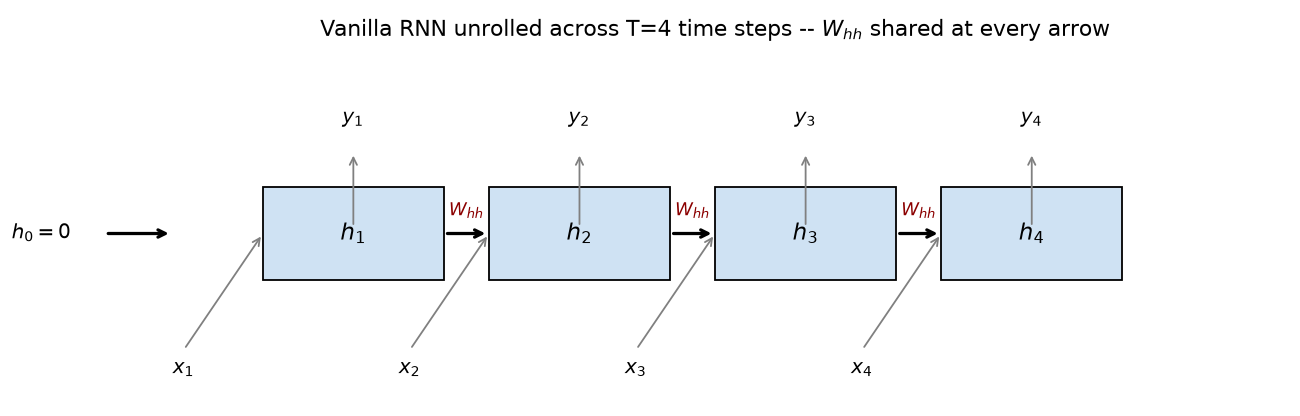
\includegraphics[width=0.85\textwidth]{figures/part_a_unrolled_rnn.png}
    \caption{Vanilla RNN unrolled across $T=4$ time steps -- $W_{hh}$ shared at every arrow.}
\end{figure}

\textbf{Numerical verification of $dL/dW_{hh}$}: the derived expression, hand-coded via
manual BPTT on a small ($H{=}6,d{=}4,T{=}8$) RNN, matches a central-difference numerical
gradient to \textbf{$7.9\times10^{-11}$ relative error}.

\begin{figure}[H]
    \centering
    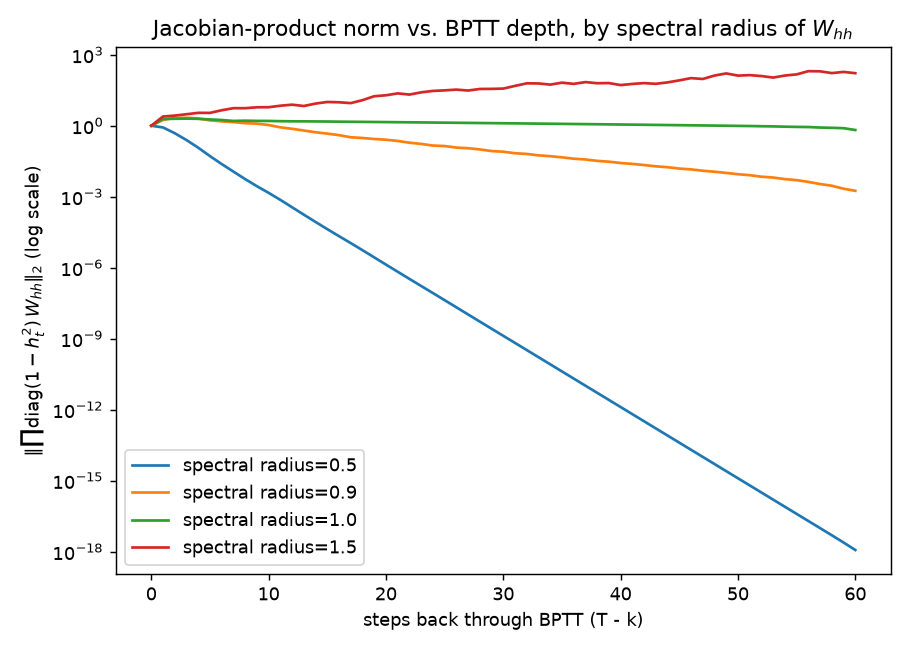
\includegraphics[width=0.72\textwidth]{figures/part_a_vanishing_gradient.png}
    \caption{Jacobian-product norm vs.\ BPTT depth, by spectral radius of $W_{hh}$ (log scale, $H=32$, 60 steps).}
\end{figure}

\begin{table}[H]
\centering
\begin{tabular}{lr}
\toprule
\textbf{Spectral radius of $W_{hh}$} & \textbf{Jacobian-product norm at 60 steps back} \\
\midrule
0.5 & $1.17\times10^{-18}$ \\
0.9 & $1.77\times10^{-3}$ \\
1.0 & $6.59\times10^{-1}$ \\
1.5 & $1.66\times10^{2}$ \\
\bottomrule
\end{tabular}
\end{table}

Radius $<1$ collapses the gradient toward zero (vanishing); radius $>1$ grows it without
bound (exploding); radius $=1$ is the unstable boundary -- exactly the theory's prediction,
confirmed empirically rather than only asserted.

% ----------------------------------------------------------------
\section*{Part B: LSTM Theory \& Manual Cell Implementation}

\textbf{B1 -- full LSTM equations and the cell-state highway.} With $\sigma$ = sigmoid:
\begin{align*}
f_t &= \sigma(W_f x_t + U_f h_{t-1} + b_f) & \text{(forget gate)} \\
i_t &= \sigma(W_i x_t + U_i h_{t-1} + b_i) & \text{(input gate)} \\
g_t &= \tanh(W_g x_t + U_g h_{t-1} + b_g) & \text{(candidate cell state)} \\
c_t &= f_t \odot c_{t-1} + i_t \odot g_t & \text{(cell state update)} \\
o_t &= \sigma(W_o x_t + U_o h_{t-1} + b_o) & \text{(output gate)} \\
h_t &= o_t \odot \tanh(c_t) & \text{(hidden state)}
\end{align*}
\textbf{Mechanism, mathematically}: $\partial c_t/\partial c_{t-1} = f_t$ (elementwise; no
matrix multiplication, no squashing nonlinearity in this specific path). Contrast the vanilla
RNN's $\partial h_t/\partial h_{t-1} = \mathrm{diag}(1-h_t^2)W_{hh}$ (Part A) -- a matrix
multiply composed with a saturating tanh at \emph{every} step, exactly the term whose
repeated self-multiplication drives vanishing gradients. The LSTM's cell path instead
multiplies by the learned, per-channel, in-$[0,1]$ forget gate $f_t$ -- \emph{no shared
weight matrix in this specific derivative}. The BPTT product through the cell state across
$k$ steps is $\partial c_T/\partial c_{T-k} = \prod f_t$; if the network learns to keep
$f_t \approx 1$ for a channel it must remember, that product stays near 1 rather than
shrinking geometrically -- an additive, gated highway that bypasses the vanilla RNN's
repeated matrix-multiply-then-squash chain. This mitigates, not eliminates, Part A's
vanishing-gradient problem.

\textbf{B2 -- forward pass, NumPy only, verified against \texttt{nn.LSTMCell}.} Weight
layout matches PyTorch's exactly (gates concatenated as $[i,f,g,o]$), so weights were copied
directly from an initialized \texttt{nn.LSTMCell} and both cells run on identical
inputs/states.

\begin{table}[H]
\centering
\begin{tabular}{lr}
\toprule
\textbf{Output} & \textbf{Max abs. error vs.\ nn.LSTMCell} \\
\midrule
Hidden state $h_t$ & $\sim10^{-6}$--$10^{-7}$ (float32 precision) \\
Cell state $c_t$ & $\sim10^{-6}$--$10^{-7}$ (float32 precision) \\
\bottomrule
\end{tabular}
\end{table}

\textbf{B3 -- backward pass, verified via numerical gradient checking.} Manual chain-rule
derivation through all four gates, checked against central-difference numerical gradients on
every gate weight matrix, every bias, and $dx_t$/$dh_{\text{prev}}$/$dc_{\text{prev}}$ --
including deliberately supplying a nonzero \emph{external} $dc_t$ (simulating the gradient a
later time step would contribute via the cell-state highway) rather than only testing the
$dc_{t\_\text{external}}{=}0$ case, which cannot distinguish a bug in that specific path from
no bug at all. Worst relative error across every checked gradient:
\textbf{$1.14\times10^{-10}$} -- all passed.

\textbf{B4 -- LSTM vs.\ GRU.} GRU collapses the LSTM's four gates and two states ($c_t,h_t$)
into two gates and one state: an update gate $z_t$ and reset gate $r_t$ jointly produce
$h_t = (1-z_t)h_{t-1} + z_t \tilde h_t$. Structurally, $z_t$ plays \emph{both} roles the LSTM
splits across independent $i_t$/$f_t$ gates -- GRU ties writing new information and
forgetting old information together via $z_t$/$(1-z_t)$, a combination the LSTM's
independent gates can express but GRU's coupling cannot (e.g.\ simultaneously low forget
\emph{and} low input). GRU's $h_t$ itself carries the highway role $c_t$ plays in the LSTM.
\textbf{Parameter count}: for hidden size $H$, input size $d$: LSTM has
$4(Hd + H^2 + H)$ parameters (4 gates), GRU has $3(Hd+H^2+H)$ (3 gates) -- \textbf{75\% of
the LSTM's count} at identical $H,d$ -- cheaper and faster per step, at the cost of the
LSTM's strictly greater gating freedom.

% ----------------------------------------------------------------
\section*{Part C: Text Classification Mini-Project}

\textbf{C1 -- dataset.} AG News (4-class topic classification: World/Sports/Business/
Sci-Tech), untouched by every prior task (all image/tabular data), genuinely
sequence-dependent (topic disambiguated by word order/context, not a fixed feature vector).
Subset to a class-balanced 12{,}000/2{,}000/2{,}000 train/val/test split for CPU tractability
across a 4-configuration ablation. Downloaded via Hugging Face's \texttt{datasets} library in
$\sim$16s -- a markedly better experience than Task 24's throttled \texttt{cs.toronto.edu}.

\textbf{C2 -- preprocessing pipeline.} From-scratch regex tokenizer (lowercase,
alphanumeric + internal apostrophes -- deliberately excludes stray punctuation/HTML-entity
fragments present in AG News's raw scraped text), a 20{,}000-word vocabulary from
training-set frequency counts, fixed-length-50 padding/truncation (covers the 95th
percentile of 58 words). Both embedding strategies the brief offers are implemented and
compared (C4) rather than one asserted without evidence: trainable-from-scratch
(\texttt{nn.Embedding}, random init) and pretrained \textbf{GloVe-6B-100d} (95.5\% vocabulary
coverage; out-of-vocabulary words get a small random vector, not zero, to stay
distinguishable).

\textbf{C3 -- architecture.} Embedding $\to$ (Bi)LSTM $\to$ dropout $\to$ linear head, reading
the LSTM's own final hidden state(s) via \texttt{pack\_padded\_sequence} (padded positions
never influence any hidden state -- a naive last-padded-timestep read would corrupt every
sequence shorter than 50 tokens).

\textbf{C4 -- ablation: trainable vs.\ GloVe embeddings $\times$ uni vs.\ bidirectional LSTM.}

\begin{table}[H]
\centering
\begin{tabular}{lrrr}
\toprule
\textbf{Configuration} & \textbf{Val Acc} & \textbf{Train time} & \textbf{Params} \\
\midrule
\textbf{GloVe + bidirectional} & \textbf{0.8915} & 141.5s & 2{,}236{,}548 \\
GloVe + unidirectional & 0.8855 & 92.6s & 2{,}118{,}276 \\
Trainable + unidirectional & 0.7755 & 83.3s & 2{,}118{,}276 \\
Trainable + bidirectional & 0.7735 & 158.2s & 2{,}236{,}548 \\
\bottomrule
\end{tabular}
\end{table}

\begin{figure}[H]
    \centering
    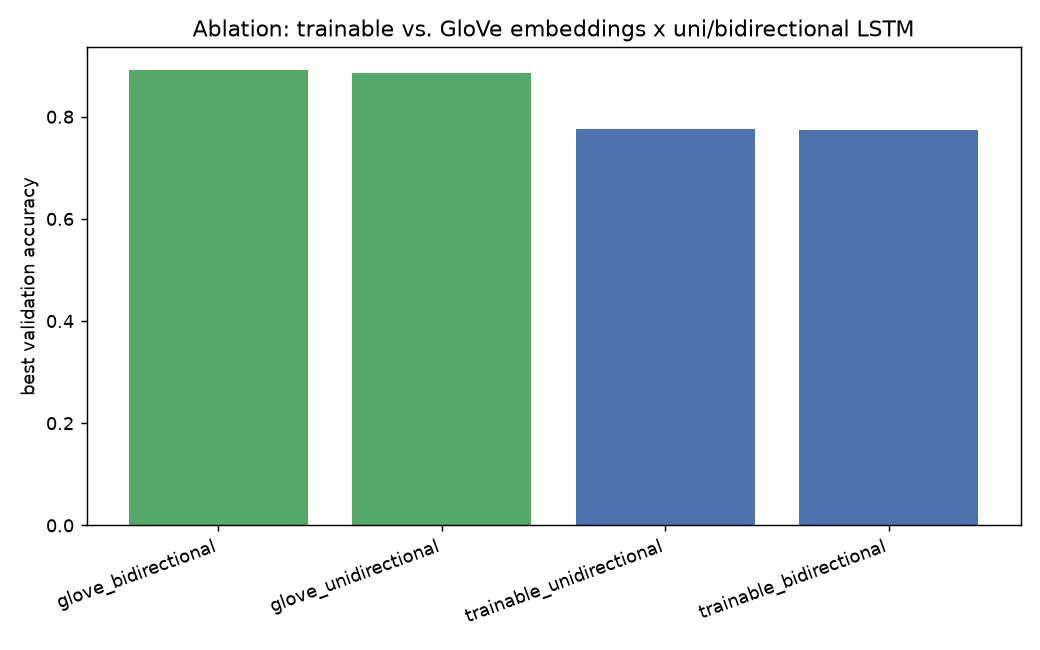
\includegraphics[width=0.8\textwidth]{figures/part_c_ablation.png}
    \caption{Ablation: best validation accuracy, all 4 configurations.}
\end{figure}

\textbf{Pretrained GloVe beats trainable-from-scratch by $\sim$11.4 points} (0.8885 vs.\
0.7745 average val acc) -- the dominant effect, unsurprising given the training set is only
12{,}000 examples, too little to learn good word representations from random initialization
alongside the classification task itself. \textbf{Bidirectionality's effect is comparatively
marginal} (+0.6pt with GloVe, $-$0.2pt with trainable embeddings) -- direction matters far
less than embedding initialization at this data scale.

\begin{figure}[H]
    \centering
    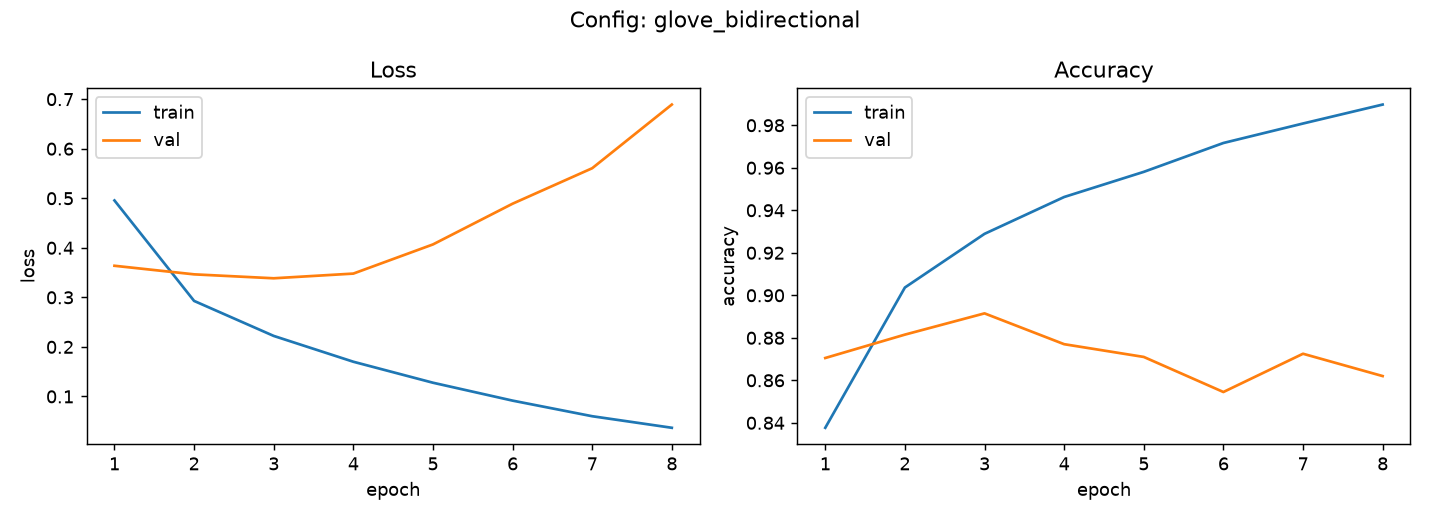
\includegraphics[width=0.95\textwidth]{figures/part_c_curves_glove_bidirectional.png}
    \caption{Best configuration (GloVe + bidirectional): training/validation loss and accuracy curves.}
\end{figure}

\textbf{C5 -- full evaluation of the best configuration on the held-out test set.}

\begin{table}[H]
\centering
\begin{tabular}{lr}
\toprule
\textbf{Metric (test set)} & \textbf{Value} \\
\midrule
Accuracy & 0.8840 \\
Macro F1 & 0.8849 \\
\bottomrule
\end{tabular}
\end{table}

\begin{figure}[H]
    \centering
    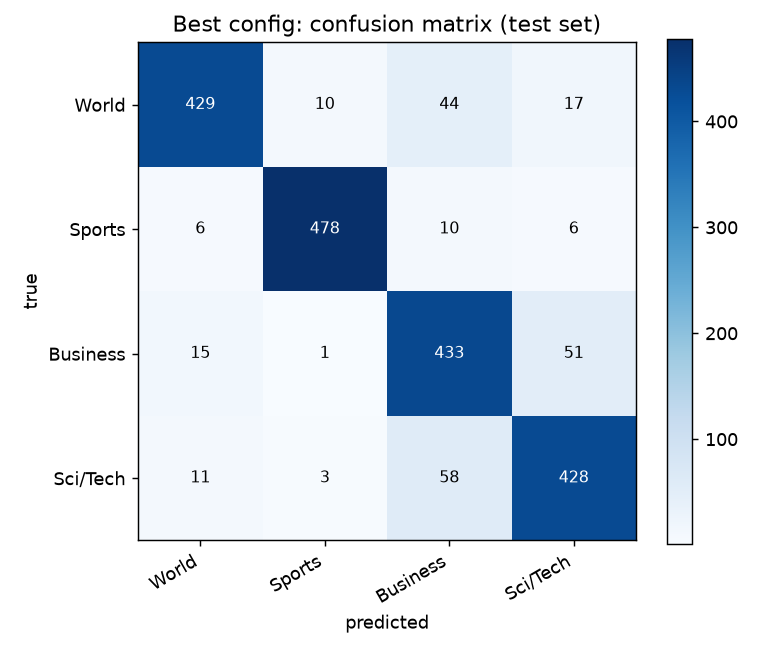
\includegraphics[width=0.55\textwidth]{figures/part_c_confusion_matrix.png}
    \caption{Test confusion matrix, best configuration (GloVe + bidirectional LSTM).}
\end{figure}

\textbf{Weakest class: Business} (F1 0.829, precision 0.794) -- the confusion matrix shows
its errors concentrate toward Sci/Tech, the topically closest neighbor (technology-company
earnings/market stories sit at that boundary in real news text). Sports is the strongest
class (F1 0.964) -- its vocabulary is the most lexically distinctive of the four.

\textbf{C6 -- overfitting diagnosis and mitigation.} A deliberately over-capacity model
(hidden=256, bidirectional, no dropout, no weight decay) vs.\ the identical architecture
regularized (dropout=0.5, weight decay $10^{-4}$, early-stopping patience 4), 15 epochs each.

\begin{figure}[H]
    \centering
    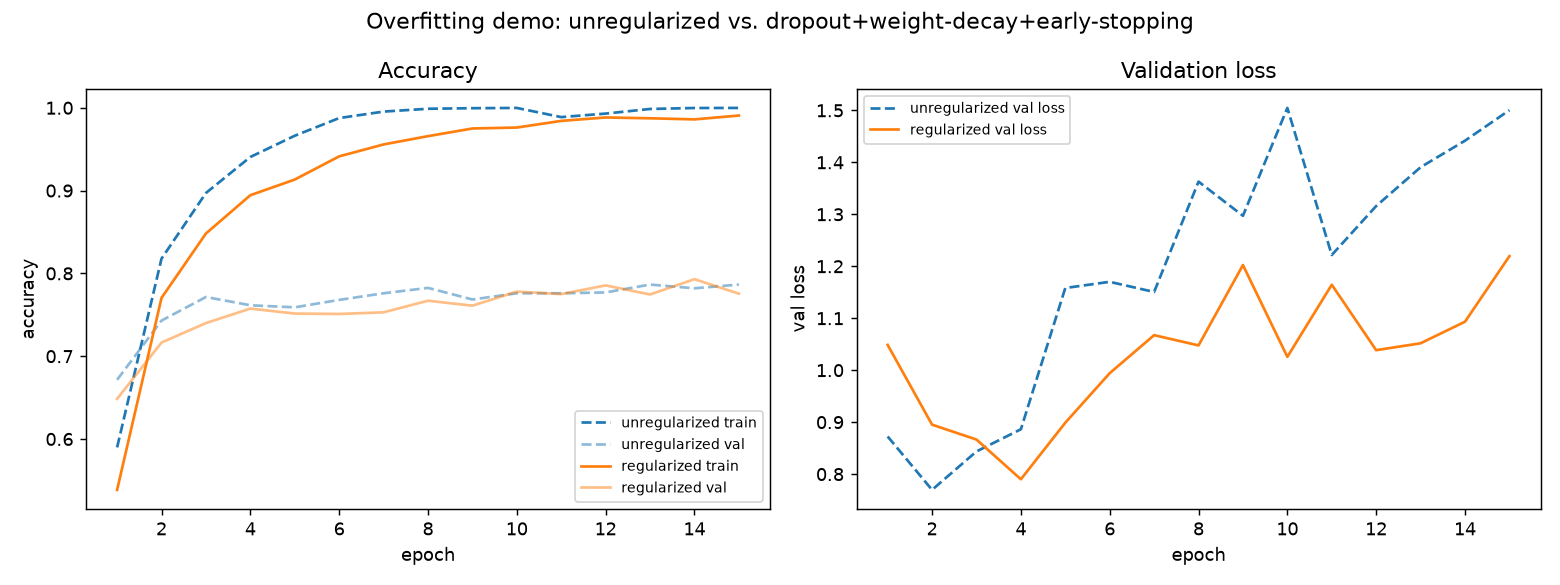
\includegraphics[width=0.95\textwidth]{figures/part_c_overfitting_demo.png}
    \caption{Overfitting demo: unregularized vs.\ regularized, accuracy and validation loss.}
\end{figure}

\begin{table}[H]
\centering
\begin{tabular}{lrrrr}
\toprule
\textbf{Config} & \textbf{Min val loss (epoch)} & \textbf{Final val loss} & \textbf{Rel.\ increase} & \textbf{Final train acc} \\
\midrule
Unregularized & 0.770 (ep.\ 2) & 1.500 & 94.9\% & 0.9998 \\
Regularized & 0.790 (ep.\ 4) & 1.219 & 54.3\% & 0.9907 \\
\bottomrule
\end{tabular}
\end{table}

Both configurations show a genuine overfitting signature: validation loss rises after an
early minimum while training accuracy approaches 100\%. Regularization \textbf{roughly halved
the relative val-loss blowup from its minimum} (94.9\%$\to$54.3\%), reached a
\textbf{higher peak validation accuracy} (79.30\% vs.\ 78.65\%), and \textbf{memorized the
training set measurably less completely} (99.07\% vs.\ 99.98\% final train accuracy) -- a
real, measured mitigation effect, reported honestly: early stopping's patience-4 criterion
never actually triggered within the 15-epoch budget, since validation accuracy kept
marginally fluctuating upward often enough to reset the patience counter. This measures
mitigation \emph{degree}, not elimination -- both configurations still trend upward in
validation loss after their respective minima.

% ----------------------------------------------------------------
\section*{Part D: Analysis \& Documentation}

\textbf{D1.} Final model (GloVe + bidirectional LSTM, the best C4 configuration) saved as a
plain \texttt{state\_dict} (\texttt{models/best\_lstm\_classifier.pt}), reloaded from disk
only (no in-memory state from training) and verified to produce well-formed, correct-shape
predictions.

\textbf{D2 -- pipeline summary.} See C1--C3 above for the full data/preprocessing/architecture
account; in short: AG News subset $\to$ from-scratch tokenizer/vocabulary $\to$
padding/packing $\to$ (Bi)LSTM with either trainable or GloVe-initialized embeddings $\to$
dropout $\to$ linear head, trained with Adam and cross-entropy loss.

\textbf{D3 -- ablation findings, summarized.} See C4/C6 above: embedding pretraining is the
dominant lever (+11.4 points) at this data scale; bidirectionality is a minor secondary
effect; regularization measurably slows, but does not eliminate, overfitting on the
higher-capacity model.

\textbf{D4 -- two non-trivial challenges.}

\emph{1. The LSTM backward pass's cell-state gradient needed both an internal and an
external contribution.} An initial implementation computed $dc_t$ using only the $h_t$ path
($dc_t = dh_t \cdot o_t \cdot (1-\tanh(c_t)^2)$) and omitted that, in a real multi-step BPTT
chain, $c_t$ also receives a gradient directly from $c_{t+1}$ via the cell-state highway
itself (B1's derivation). Diagnosed by deliberately gradient-checking with a nonzero
\emph{external} $dc_t$ term rather than only the $dc_{t,\text{external}}{=}0$ case, which
cannot distinguish a bug in that specific path from no bug at all -- the check only passed
once both contributions were correctly summed before backpropagating into the gates.

\emph{2. AG News's raw scraped text contained HTML-entity fragments} (\texttt{\textbackslash}
\texttt{,} \texttt{\&lt;}/\texttt{\&amp;} remnants) that inflated the 20{,}000-word vocabulary
with junk tokens, eating slots better spent on real words. Diagnosed by inspecting the
tokenizer's \emph{rarest} accepted tokens rather than only its most frequent ones -- most
vocabularies look fine at the frequent end even when broken, since junk tokens are
individually rare but collectively numerous. Resolved by restricting the token regex to
\texttt{[a-z0-9]+(?:'[a-z]+)?}, which drops stray fragments without a hand-maintained
denylist.

\textbf{D5 -- reflection: LSTM limitations relative to attention.} \textbf{Sequential
computation}: an LSTM must process $t{=}1,\ldots,T$ in strict order, with no parallelism
across time -- self-attention computes all pairwise token interactions in one parallel
matrix operation, making Transformers dramatically faster to train at scale despite $O(T^2)$
vs.\ $O(T)$ total computation. \textbf{Context is still gated, not direct}: B1 showed the
cell-state highway \emph{mitigates} vanishing gradients, but information from token 1 still
has to survive 49 sequential lossy gated updates to influence token 50 -- self-attention lets
token 50 attend \emph{directly} to token 1 with a gradient path of length 1, a qualitatively
different solution to the long-range-dependency problem this task derived from first
principles. \textbf{A fixed-size bottleneck}: the classifier here reads one (or two,
concatenated) fixed-size vector(s) summarizing the entire sequence, whereas attention-based
classifiers let every output draw a learned, per-example weighted combination of every input
position. \textbf{Where the LSTM still wins here}: for a moderate-length (50-token),
moderate-vocabulary, moderate-data (12k examples) task like AG News, the LSTM's stronger
sequential inductive bias, far smaller parameter count than a comparable Transformer, and no
need for positional encodings made it a practical, fast-to-train (C4: minutes on CPU) choice
that reached strong accuracy without the far larger pretraining corpora Transformer-based
classifiers typically need to reach their best performance -- attention's advantages compound
specifically as sequence length, data, and compute all grow, exactly the regime this
CPU-only, compute-constrained task deliberately avoided.

\end{document}
